\subsection{DBSP and the Unsoundness of the FirstZero Strategy}\label{sec:overview-problem}

To lay the groundwork for the problems that we address, we first discuss how DBSP implements and incrementalizes the Datalog query for transitive closure (\secref{sec:intro}) in three steps.
DBSP uses \textit{circuits} to express computations. It first compiles the query into a
``\emph{naive}'' circuit, then optimizes it into a ``\emph{semi-naive}'' circuit, and
finally optimizes it further into a ``\emph{delta-of-deltas}'' circuit. What matters for
our purposes is what is computed incrementally in these circuits;
\Cref{fig:ivm-three-steps} depicts the intermediate results of the evaluation
for one graph and one update to it.
In the figure, the vertical dimension represents changes to the input, i.e., the \emph{outer} iterations for incremental computation (e.g., we add a green edge to the first input $G_0$ to get the second input $G_1$), while the horizontal dimension represents the \emph{inner} iterations for fixpoint computation (e.g., we apply the single-step query $F$ to $G_0$ to get $G_0^1$).
The goal after each outer iteration $m$ is to obtain the transitive-closure
``view'' for graph $G_m$.

The \textbf{naive}
strategy is not optimized for incremental computation at all:
for each outer iteration, it re-runs the entire fixpoint computation from scratch;
on each inner iteration, it merely applies the non-recursive query $F$ to intermediate results (until the inner-iteration fixpoint is obtained).
Its intermediate result in the $n^{\textit{th}}$ inner iteration of the $m^{\textit{th}}$ outer iteration $G_m^n$
is the set of pairs of nodes whose distance is within $n+1$ in $G_m$.

The \textbf{semi-naive} strategy optimizes the naive strategy along the horizontal dimension (inner iterations).
The name
comes from the Datalog semi-naive evaluation strategy (Algorithm 2 from the book~\cite{Greco2015DatalogAL}).
It computes inner-iteration \emph{deltas}
of the intermediate results of the naive strategy (e.g., $G_0^{\Delta 1} = G_0^1 - G_0$ contains only the blue edge).
The intermediate result $G_m^{\Delta n}$, for $n \geq 1$, consists of
pairs of nodes whose distance is exactly $n+1$ in $G_m$.
In each outer iteration, when the inner-fixpoint is reached,
the intermediate results can be collected---e.g., $G_1 \cup G_1^{\Delta 1} \cup G_1^{\Delta 2}$---to obtain the final result.


The \textbf{delta-of-deltas} strategy further incrementalizes the semi-naive strategy
along the outer iterations
by computing \emph{outer-iteration deltas of the inner-iteration deltas}
(e.g., $\Delta G_{1}^{\Delta 1} = G_1^{\Delta 1} - G_0^{\Delta 1}$ contains only the yellow edge).
For each outer iteration, it accepts the delta of the input graph (e.g., $\Delta G_1$), and upon 
obtaining the inner fixpoint, the inner-iteration intermediate results can be collected to obtain the delta of the transitive-closure view.
For instance, for outer iteration 1, the delta of the view is the three pairs in $\Delta G_1 \cup \Delta G_1^{\Delta 1} \cup \Delta G_1^{\Delta 2}$.
Note that this value equals $G_1^2 - G_0^2$.

\begin{figure}[!tb]
    \centering
    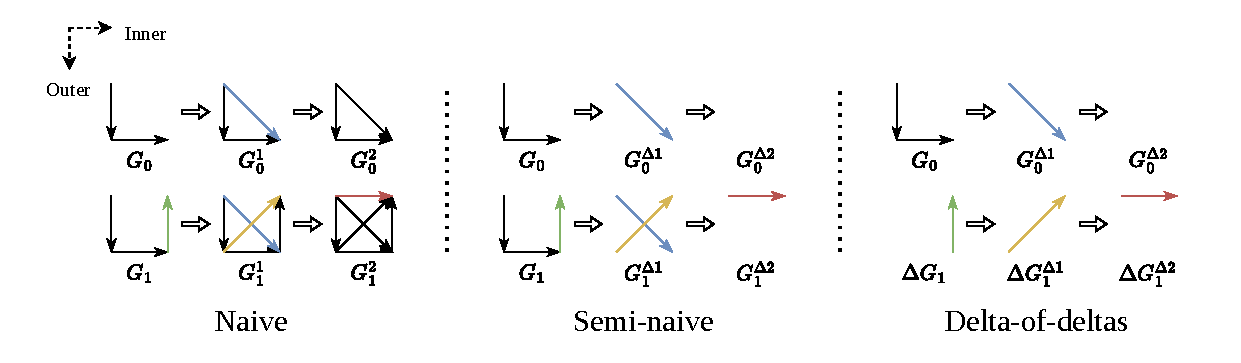
\includegraphics[width=\linewidth]{figures/three_approaches.pdf}
    \vspace{-4.0ex}
    \caption{Intermediate-evaluation results 
    arising in the three DBSP strategies for incrementalizing a transitive-closure
    query.}\label{fig:ivm-three-steps}
\end{figure}

To produce correct answers, all three strategies
need a common component we call \emph{Fixpoint Detection} (FPD): a runtime mechanism to
detect whether an inner-iteration computation has already reached a fixpoint, at which point, it can terminate the current inner iteration, collect
the intermediate results (for the semi-naive and delta-of-deltas strategies), and proceed to the next outer iteration.

In the DBSP theory,
FPD and inner-iteration collection is encapsulated in
a mathematical operator called \emph{stream elimination}, denoted by $\elim$, which takes an infinite stream $ s \in (\stream{A} := \N \to A)$ representing the intermediate results of an
\emph{unbounded} iterative computation, and produces a scalar value $a \in A$ representing the integrated final result. Intuitively, $\elim(s)$ is defined to return the sum of all \emph{non-zero} elements in $s$.
$\elim$ can only be defined as a \emph{partial} function:
it only produces an answer for
streams that have a \emph{finite} number of non-zero elements (in which case we say
that $\elim(s)$ converges).
When $\elim(s)$ diverges, the implementation can simply run forever or terminate after a timeout.
Either is semantically consistent:
DBSP is designed to be Turing-complete~\cite{budiu2025dbsp} due to unbounded loops.
The question that really matters is ``how can the system detect when a stream $s$
is all zeros beyond some point?'' in which case $\elim(s)$ indeed converges, and the semantics demands that the answer be produced.
The challenge is that the implementation has only a finite prefix of $s$ at run
time, and it must concretely decide all subsequent values of $s$ are zero, but
there are infinitely many of them. Finding a way to establish $s$ has finitely
many non-zero values based on a finite prefix is the essence of
the \textbf{FPD problem} in DBSP.

In the DBSP paper~\cite{budiu2025dbsp}, the authors suggest that for many practical queries including the Datalog queries,  $\elim$ can be ``approximated without loss of precision by integrating until it encounters the first $0$''. We call this 
criterion for deciding convergence the FirstZero criterion (or FirstZero strategy).

For the naive and the semi-naive strategies,\footnote{
  In the DBSP circuit for the naive strategy,
  the intermediate results are in fact first differentiated to become deltas and then sent to $\elim$, so the input to $\elim$ is the same in
  the circuits for the naive and semi-naive strategies.
}
the FirstZero criterion is indeed a sound criterion,
because the first zero in the delta stream ($G_m^{\Delta n} = 0$) implies that the fixpoint of the original stream has been reached ($G_m^{n} = F(G_m^{n-1}) = G_m^{n-1}$), so
$G_m^{\Delta p}$, for $p \geq n$
must all be zero.

\begin{figure}[!tb]
    \centering
    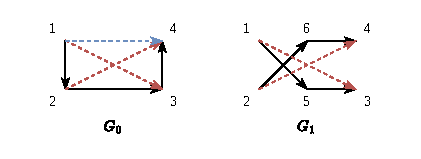
\includegraphics[width=0.46\linewidth]{figures/counterexample.pdf}
    \vspace{-4.0ex}
    \caption{
    A pair of input graphs that demonstrate that the FirstZero criterion applied to the delta-of-deltas strategy computes an incorrect answer.
    Instead of the correct transitive closure of $G_1$, namely, $\{ (1,5), (2,6), (5,3), (6,4), \textcolor{red}{(1,3)}, \textcolor{red}{(2,4)} \}$, we would obtain $\{ (1,5), (2,6), (5,3), (6,4), \textcolor{red}{(1,3)}, \textcolor{red}{(2,4)}, \textcolor{blue}{(1,4)} \}$.
    }\label{fig:counterexample}
\end{figure}

However, for the delta-of-deltas strategy, the FirstZero criterion is, in
general, incorrect. That is, if a runtime executes the stream
elimination operator $\elim$ in a DBSP operator by summing until the first zero,
it produces an incorrect result on some inputs where there are more non-zero
elements that should be summed; there is a convergence point in the input, but it is further
ahead in the stream than the first zero.

For a concrete example where FirstZero produces an incorrect answer, consider the two graphs $G_0$ and $G_1$ shown in Fig.~\ref{fig:counterexample}.
In DBSP, the delta between two databases can have negative quantities, representing deletions.
For $G_0$ and $G_1$, the delta $\Delta G_1$ consists of negative edges $\{ (1,2), (2,3), (3,4) \}$ and positive edges $\{ (1,5), (2,6), (5,3), (6,4) \}$.
Note that after the first step of the semi-naive strategy, $G_0^{\Delta 1}$ and $G_1^{\Delta 1}$ are exactly the same (the positive red edges $\{ \textcolor{red}{(1,3)}, \textcolor{red}{(2,4)} \}$).
Consequently, after the first step of the delta-of-deltas strategy, $G_0^{\Delta 1}$ consists of $\{ \textcolor{red}{(1,3)}, \textcolor{red}{(2,4)} \}$ and $\Delta G_{1}^{\Delta 1} = G_1^{\Delta 1} - G_0^{\Delta 1} = \emptyset$ (because subtraction operates over $\mathbb{Z}$-sets, elements with identical positive counts cancel out)---i.e., it is the first zero, so the FirstZero criterion would say, incorrectly, that the inner-iteration fixpoint for $\Delta G_1$ has been reached.



When the delta-of-deltas strategy is properly performed, $\Delta G_1^{\Delta 1}$ is $\emptyset$, but the subsequent $\Delta G_1^{\Delta 2}$ is not $\emptyset$:
$G_0^{\Delta 2}$ consists of the blue edge $\{ \textcolor{blue}{(1,4)} \}$, and thus $\Delta G_1^{\Delta 2}$ consists of the \emph{negative} blue edge $\{ \textcolor{blue}{(1,4)} \}$.
Only when we get to $G_0^{\Delta 3}$ and $\Delta G_1^{\Delta 3}$ do we have $\emptyset$ at corresponding inner-iteration spots of both outer iterations.
The collected inner-iteration intermediate results are
$\Delta G_1 \cup \Delta G_1^{\Delta 1} \cup \Delta G_1^{\Delta 2} \cup \Delta G_1^{\Delta 3}$, which has negative edges $\{ (1,2), (2,3), (3,4), \textcolor{blue}{(1,4)} \}$ and positive edges $\{ (1,5), (2,6), (5,3), (6,4) \}$.
When combined with the transitive closure of $G_0$, i.e., positive edges $\{ (1,2), (2,3), (3,4), \textcolor{red}{(1,3)}, \textcolor{red}{(2,4)}, \textcolor{blue}{(1,4)} \}$, we obtain the transitive closure of $G_1$, $\{ (1,5), (2,6), (5,3), (6,4), \textcolor{red}{(1,3)}, \textcolor{red}{(2,4)} \}$.

In contrast, the FirstZero criterion produces an incorrect result.
The collected inner-iteration intermediate results are
$\Delta G_1 \cup \Delta G_1^{\Delta 1}$, which has negative edges $\{ (1,2), (2,3), (3,4) \}$ and positive edges $\{ (1,5), (2,6), (5,3), (6,4) \}$.
When combined with the transitive closure of $G_0$, i.e., positive edges $\{ (1,2), (2,3), (3,4), \textcolor{red}{(1,3)}, \textcolor{red}{(2,4)}, \textcolor{blue}{(1,4)} \}$, we obtain the incorrect result $\{ (1,5), (2,6), (5,3), (6,4), \textcolor{red}{(1,3)}, \textcolor{red}{(2,4)}, \textcolor{blue}{(1,4)} \}$, which has the extra positive edge $\textcolor{blue}{(1,4)}$.

\subsection{Overview of Our Theory}\label{sec:overview-solution}

The counter-example to FirstZero in \secref{sec:overview-problem}, together with the undecidability result in \secref{sec:fpd-undecidability}, reveals a gap between the mathematical theory of DBSP and its practical implementation. Our theory addresses this gap through a simple progression: specify convergence mathematically, strengthen that specification to require internal stability, and turn internal stability into a runtime check. This progression operates at two scales---locally for one iterative computation and globally for a complete circuit.

To express these two scales uniformly, we define a core calculus of well-formed DBSP circuits (\secref{sec:pre-language}). In this calculus, $\delta_0$ initiates an unbounded iterative computation and $\elim$ integrates its result; we call the circuit between them a \emph{bracketed circuit}. The Fixpoint Detection (FPD) problem asks when one such bracketed circuit reaches a fixpoint. A complete circuit may contain multiple, potentially nested bracketed circuits, so the global \emph{Convergence Detection} problem asks when every bracketed sub-circuit reaches a fixpoint. We formalize both problems and show that exact FPD is undecidable for arbitrary circuits with expressive primitive nodes (\secref{sec:fpd}). The result does not apply to Datalog or regular circuits, for which our later completeness theorems yield exact detection.

Fig.~\ref{fig:intconv-overview} organizes the local and global problems into three layers. At the specification layer, \emph{external fixpoint} (ExtFP) says that a circuit's input and output are fixed after a specified iteration; when the fixed output is $0$, ExtFP is equivalent to the original FPD specification. Its global counterpart, \emph{external convergence} (ExtConv), requires every bracketed sub-circuit to converge. At the criterion layer, inspired by the internal-state-stability criterion used in Feldera~\cite{feldera_repo}, \emph{internal fixpoint} (IntFP) strengthens ExtFP by requiring every internal node to reach an external fixpoint, and \emph{internal convergence} (IntConv) requires the inner circuit of every bracketed sub-circuit to satisfy IntFP with fixed output $0$. Consequently, IntFP implies ExtFP and IntConv implies ExtConv (\secref{sec:intfp}). At the detection layer, \emph{state fixpoint} (StFP) connects the internal criterion to the state-oriented check performed at runtime.

\begin{figure}[!tb]
    \centering
    \begin{subfigure}[b]{0.58\textwidth}
        \centering
        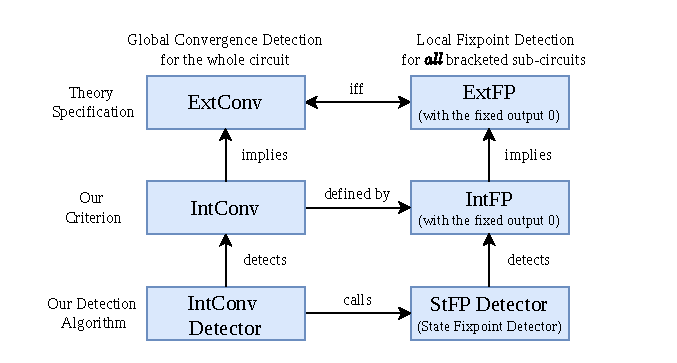
\includegraphics[width=\linewidth]{figures/overview1.pdf}
        \caption{Overview of the IntConv theory.}\label{fig:intconv-overview}
    \end{subfigure}
    \hfill
    \begin{subfigure}[b]{0.40\textwidth}
        \centering
        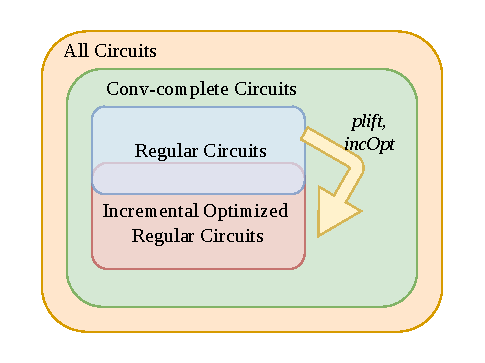
\includegraphics[width=\linewidth]{figures/overview2.pdf}
        \caption{Overview of the Conv-complete circuits.}\label{fig:conv-complete-overview}
    \end{subfigure}
    \caption{Overview of the concepts that play a role in our theory.}\label{fig:overview}
\end{figure}

The distinction between external and internal convergence also provides theoretical evidence for implementation benefits of IntConv. At the end of \secref{sec:intfp}, we give a data-dependency example in which an evaluation that relies only on ExtConv can require recursive trace-backs and additional retained state. This is a qualitative example, not an empirical performance evaluation or a general lower bound.

We show that IntConv is indeed detectable using StFP and a high-level detector (\secref{sec:detector}). Although our denotational semantics treats circuits as pure functions, implementations maintain state; StFP asks whether the circuit would be at an internal fixpoint if its observed input remained fixed. We give a structural StFP detector that is sound and complete for StFP. Together with a fixed-input check, it yields a local IntFP detector. The sound and complete global IntConv detector applies this local detector to every bracketed sub-circuit and checks that the fixed output is $0$. Because the StFP detector follows circuit structure, it also applies uniformly to nested bracketed circuits. We will compare this capability with the Feldera implementation in \secref{sec:related}.

Finally, we identify useful classes of circuits on which the internal and external specifications coincide as shown in Fig.~\ref{fig:conv-complete-overview}. We call a circuit \emph{convergence-complete} (Conv-complete) when its ExtConv implies IntConv for every input. On these circuits, the implementable internal criterion exactly matches the mathematical external convergence specification. We use \emph{regular circuits} as a name for the standard DBSP recursive sublanguage generated by lifted scalar circuits, sequential and parallel composition, Datalog queries, and while queries, including their nested uses. We prove that regular circuits are Conv-complete. We also formalize DBSP's incremental optimization as the syntax-directed transformations $\mathsf{plift}$ and $\mathsf{incOpt}$ and prove that both preserve Conv-completeness, yielding the classes summarized in Fig.~\ref{fig:conv-complete-overview} (\secref{sec:useful}).
